%\documentclass[10pt,a4paper]{article}
\documentclass[12pt,a4paper]{article}
\usepackage{graphicx,amsmath}
%\usepackage{subfigure}
\usepackage{float}
\usepackage[german]{babel}
\usepackage[utf8]{inputenc}
\setcounter{secnumdepth}{4}
\usepackage[top=2cm, bottom=2.5cm, left=3cm, right=3cm]{geometry}
\begin{document}


%\title{Bachelorarbeit}
%\author{Richard Kullmann}
%\date{02.06.2017}

\thispagestyle{empty}
%\setcounter{page}{2}
\newpage
\tableofcontents
\thispagestyle{empty}
\newpage
\pagenumbering{arabic}
\section{Modell}
Es wird das $I_{Na,p}+I_K$-Modell mit additivem Rauschen betrachtet:

\begin{align*}
C\dot{V} &= I - g_L(V-E_L) - g_{Na}m_{\infty}(V)(V-E_{Na}) - g_Kn(V-E_K)+\sqrt{2D}\xi(t)\\
\dot{n} &= (n_{\infty}(V)-n)/\tau(V)
\end{align*}
Dabei ist $m_{\infty}$ die Aktivierungsvariable des instantanen $Na^+$-Stromes, während $n$ den langsameren $K^+$-Strom reguliert. Die Steady-State-Aktivierungsfunktionen wurden durch eine Boltzmann-Kurve angenähert:
\begin{align*}
f_{\infty}(V) = \frac{1}{1+\exp\{(V_{1/2}-V)/k\}}
\end{align*}
Für die Parameter wurden folgende Werte verwendet:\\\\
$C=1$ , $g_L=8$ , $E_L=-80$ , $g_{Na}=20$ , $E_{Na}=60$ , $g_K=9$ , $E_K=-90$.
\begin{align*}
\intertext{Instantaner $Na^+$-Strom:} &k_m=15 , V_{1/2,m}=-20. 
\\
\intertext{$K^+$-Strom:} &k_n=5 , V_{1/2,n}=-25 , \tau(V)=0.152.
\end{align*}
\section{optimaler Zeitschritt}
Wie aus den noise-getriebenen Simulationen noch nicht hervorging, hat die Untersuchung des deterministischen Modells ($D=0$) gezeigt, dass die ursprüngliche Schrittweite von $5*10^{-4}$ noch nicht die optimale Genauigkeit erreichen konnte:
\begin{figure}[H]
\centering
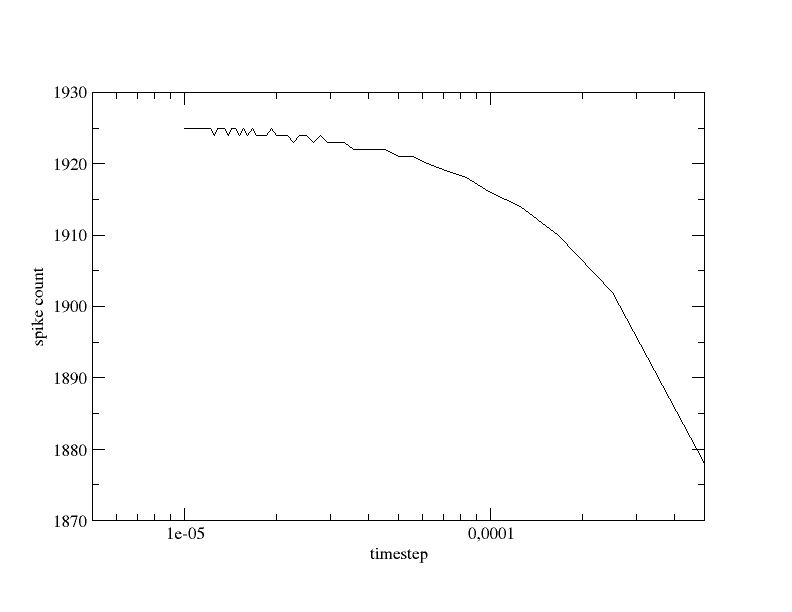
\includegraphics[scale=0.4]{timestep.png} 
\caption{Eine Verringerung des Zeitschritts kann die Genauigkeit noch einmal und ca 3\% steigern}
\label{ts}
\end{figure}
Wie stark sich das auswirkt, kann am besten am Verlauf der Membranspannung beobachtet werden, wenn das Neuron dauerhaft feuert:
\begin{figure}[H]
	\centering
	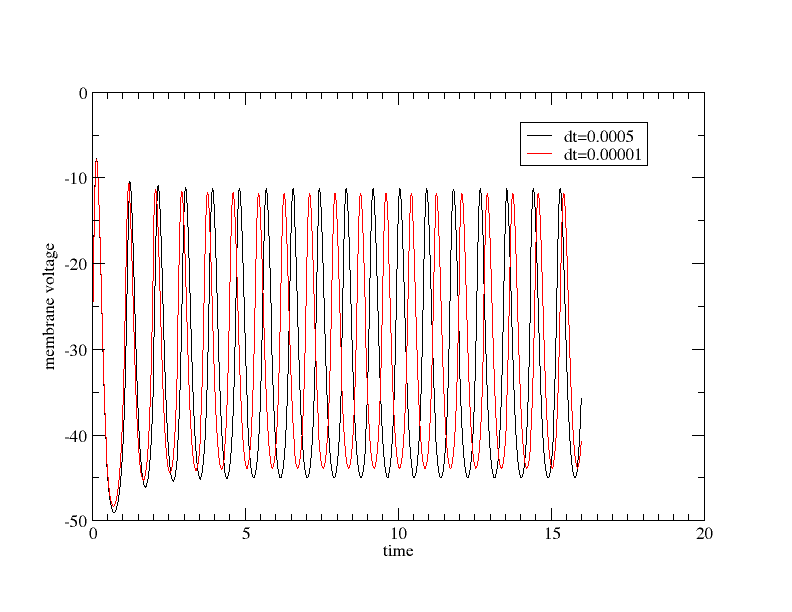
\includegraphics[scale=0.4]{spikecount.png} 
	\caption{Die erhöhte Frequenz bei kleinerem Zeitschritt ist deutlich zu erkennen}
	\label{sc}
\end{figure}
Also habe ich alle Rechnungen mit kleineren Zeitschritten wiederholt. 
\section{Phasenportraits}
Zunächst ging es an die Veranschaulichung des Phasenportraits. Dafür wurde für verschiedene Kombinationen von Startparametern die Anzahl der Spikes in einer kurzen Zeitspanne gezählt, sodass sich Werte in der Größenordnung $10^{1}$ ergaben.
\\
Die Phasenportraits wurden für verschiedene Ströme $I$ zwischen -1 und 5 erzeugt.
Der blaue Punkt markiert jeweils den Gleichgewichtszustand.
\begin{figure}[H]
	\centering
	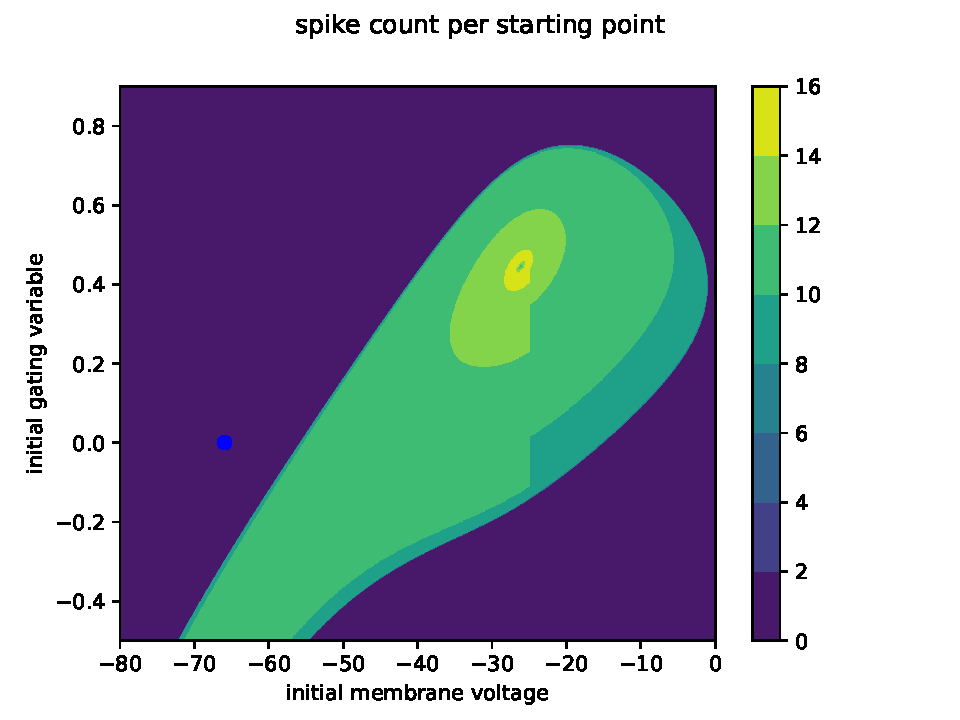
\includegraphics[scale=0.9]{contourneu-1neu.pdf} 
	\caption{Phasenportrait für $I=-1$}
	\label{ppm1}
\end{figure}
\begin{figure}[H]
	\centering
	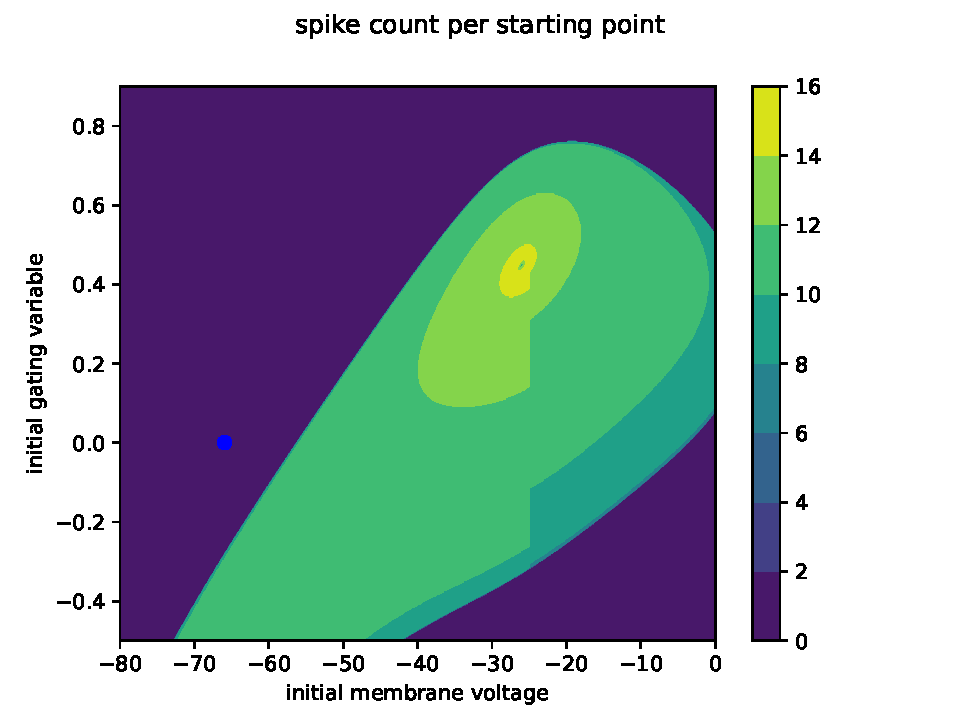
\includegraphics[scale=0.9]{contourneu0neu.pdf} 
	\caption{Phasenportrait für $I=0$}
	\label{pp0}
\end{figure}\begin{figure}[H]
\centering
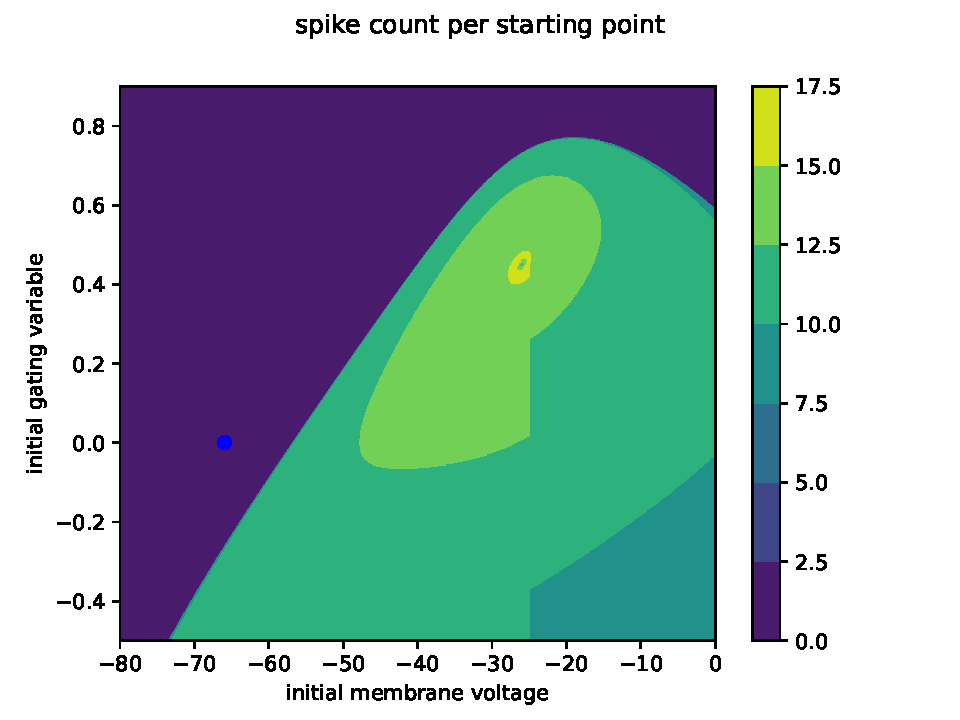
\includegraphics[scale=0.9]{contourneu1neu.pdf} 
\caption{Phasenportrait für $I=1$}
\label{pp1}
\end{figure}\begin{figure}[H]
\centering
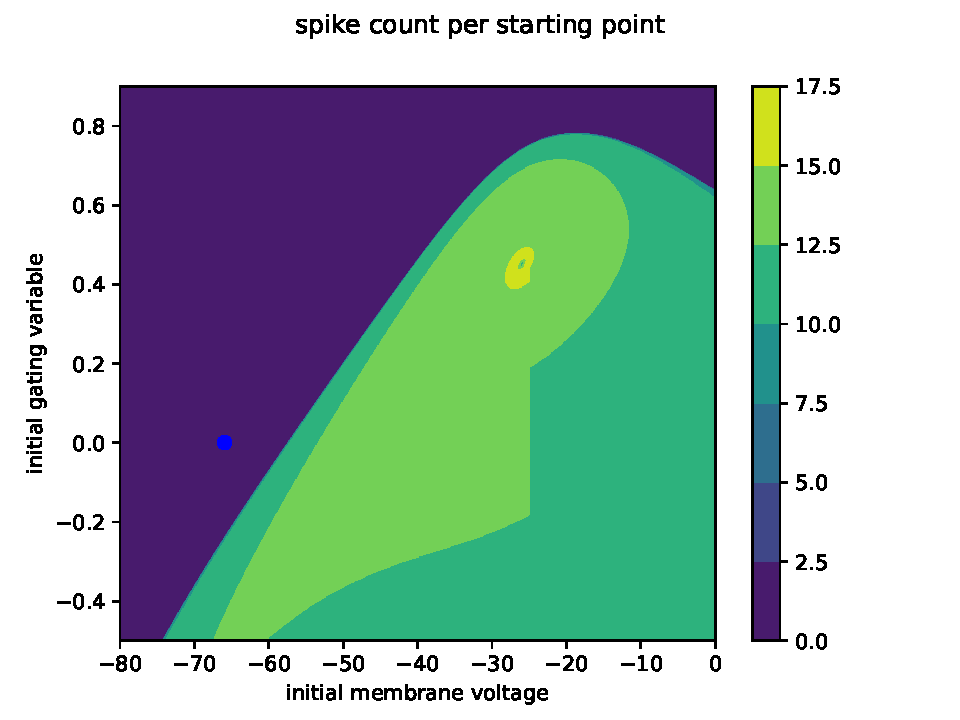
\includegraphics[scale=0.9]{contourneu2neu.pdf} 
\caption{Phasenportrait für $I=2$}
\label{pp2}
\end{figure}\begin{figure}[H]
\centering
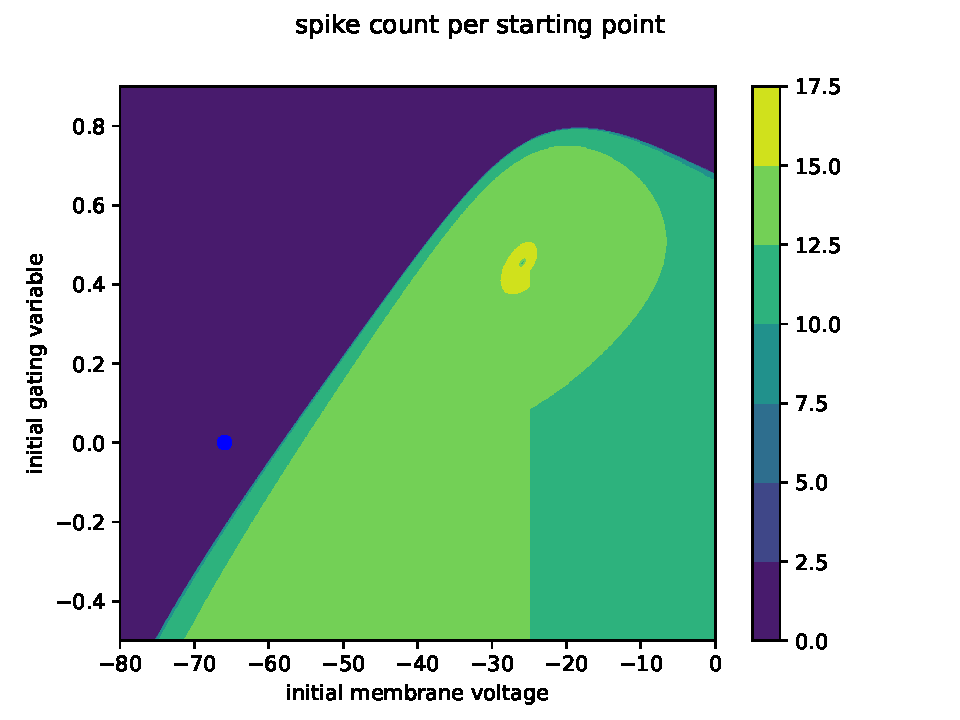
\includegraphics[scale=0.9]{contourneu3neu.pdf} 
\caption{Phasenportrait für $I=3$}
\label{pp3}
\end{figure}\begin{figure}[H]
\centering
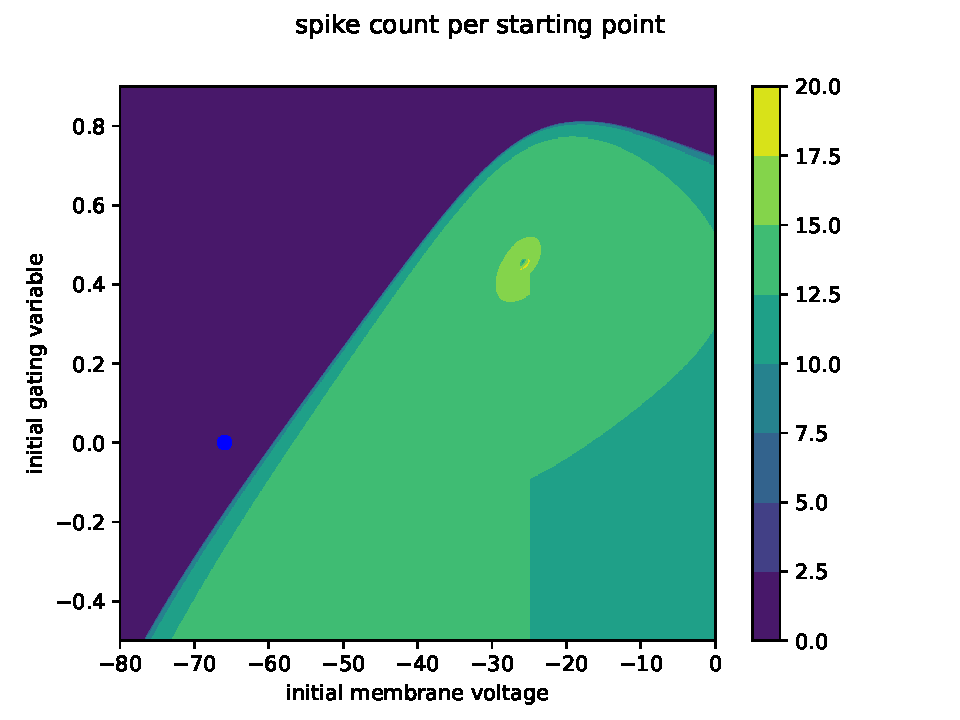
\includegraphics[scale=0.9]{contourneu4neu.pdf} 
\caption{Phasenportrait für $I=4$}
\label{pp4}
\end{figure}\begin{figure}[H]
\centering
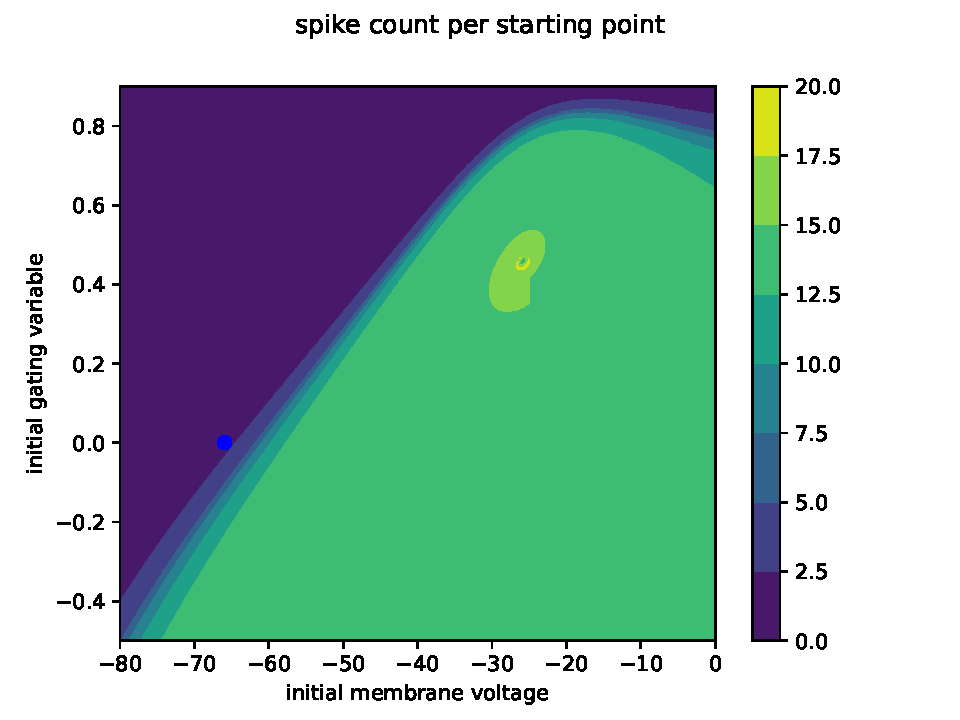
\includegraphics[scale=0.9]{contourneu5neu.pdf} 
\caption{Phasenportrait für $I=5$}
\label{pp5}
\end{figure} 
Die (scheinbare) Unstetigkeit im Plot resultiert aus der Tatsache, dass als gewähltes Kriterium das Überschreiten der Spannung $V_{th}=-25$ von unten als Spike in die Statistik eingeht. Kurven, die also leicht darüber lagen und danach feuern würden, haben also ebenfalls einen Spike ausgeführt, dieser wurde allerdings nicht gezählt, was für unsere Zwecke jedoch nicht von Belang ist.\\
Es ist deutlich zu erkennen, dass sich mit steigendem $I$ die Trajektorie im Phasenraum immer weiter ausdehnt, und wie erwartet der stabile Gleichgewichtspunkt immer näher an den Grenzwertzyklus rückt. Dementsprechend nimmt die nötige Störung für einen Wechsel zwischen ruhend/feuernd auch immer weiter ab.
\\\\
Probleme: Da der Verlauf des Grenzwertzyklus (bisher) nur numerisch bestimmt wird, ist schwer zu erkennen, wann ein Neuron diesen Zyklus erreicht hat, alsosozusagen die "Konvergenz-Zeit". Außerdem nur 'Schwarz/weiß-Bild' des Phasenraums, Lösung: einzelne Phasenraumtrajektorien plotten? 
\section{Fano-Faktor im Neuronenmodell}
Wie bereits vorher erwähnt, wurden alle Rechnungen noch einmal mit kleineren Zeitschritten wiederholt. Leider haben sich hier einige Probleme ergeben. Trotz langer Laufzeiten haben die Graphen starke Schwankungen gezeigt:
\begin{figure}[H]
	\centering
	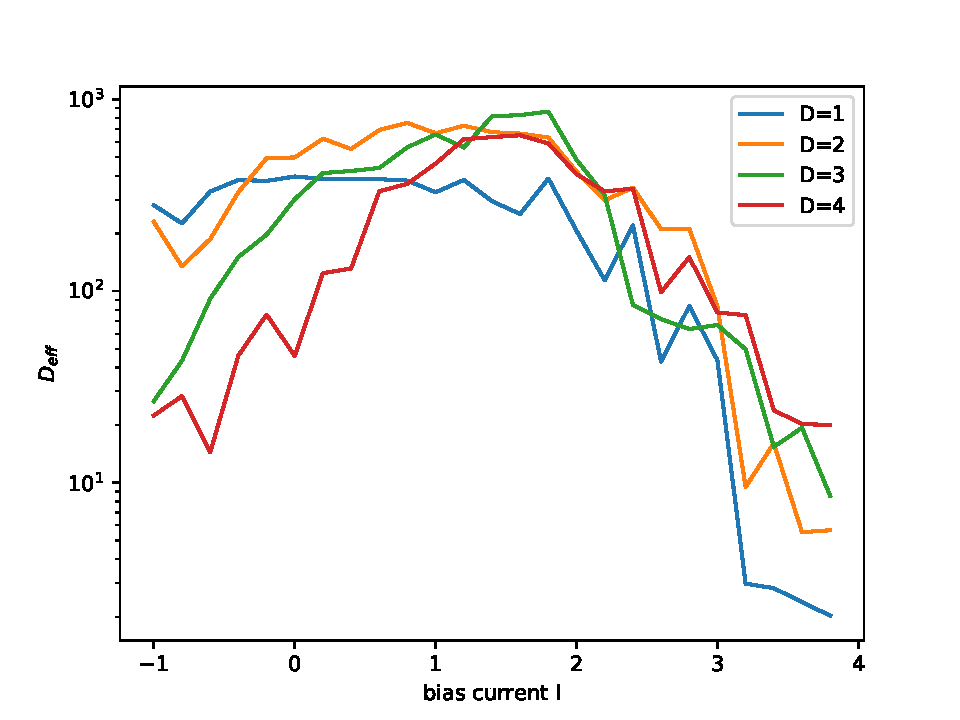
\includegraphics[scale=0.9]{dneurs.pdf} 
	\caption{Diffusionskoeffizienten}
	\label{dnc}
\end{figure} 
\begin{figure}[H]
	\centering
	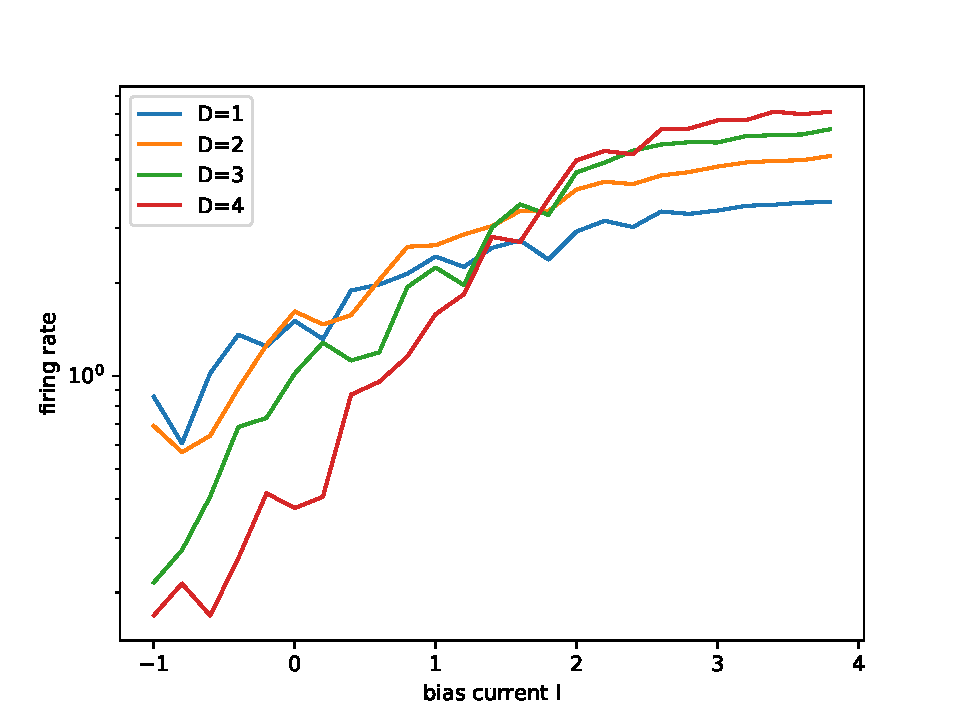
\includegraphics[scale=0.9]{gneurs.pdf} 
	\caption{Feuerraten}
	\label{gnc}
\end{figure} 
\begin{figure}[H]
	\centering
	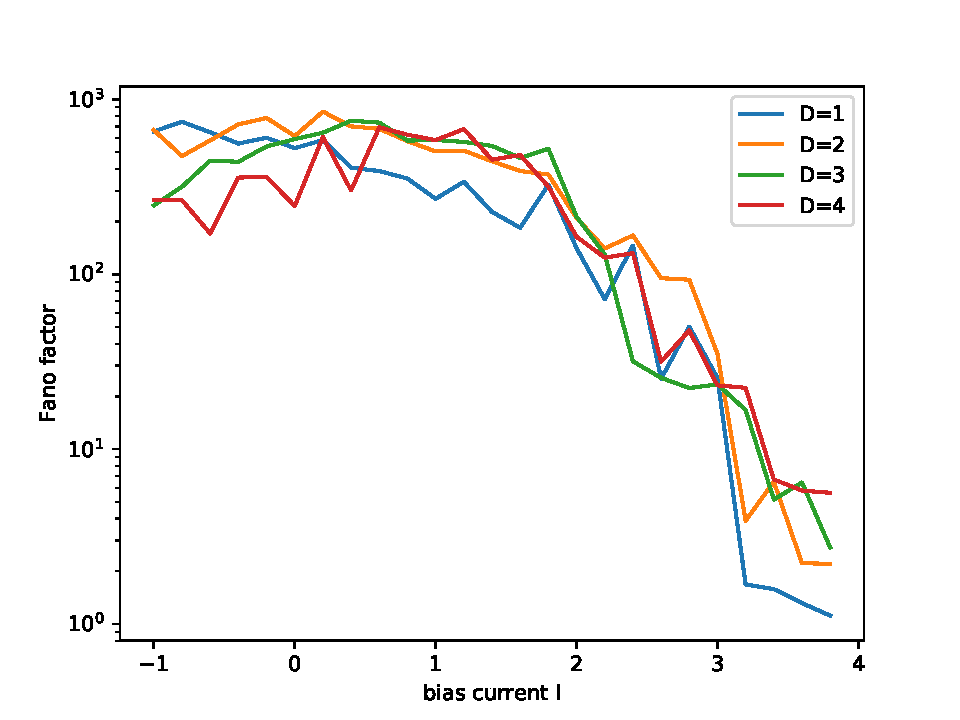
\includegraphics[scale=0.9]{fneurs.pdf} 
	\caption{Fano-Faktoren}
	\label{fnc}
\end{figure} 
Es hat sich herausgestellt, dass bei einzelnen Neuronen so viele Spikes gezählt wurden, dass der Maximalwert einer Variable überstiegen wurde. Daher habe ich statt der Laufzeit die Anzahl der Neuronen erhöht. Dies hat bei geringerer Rechnungsdauer eine deutliche Verbesserung gezeigt:

\begin{figure}[H]
	\centering
	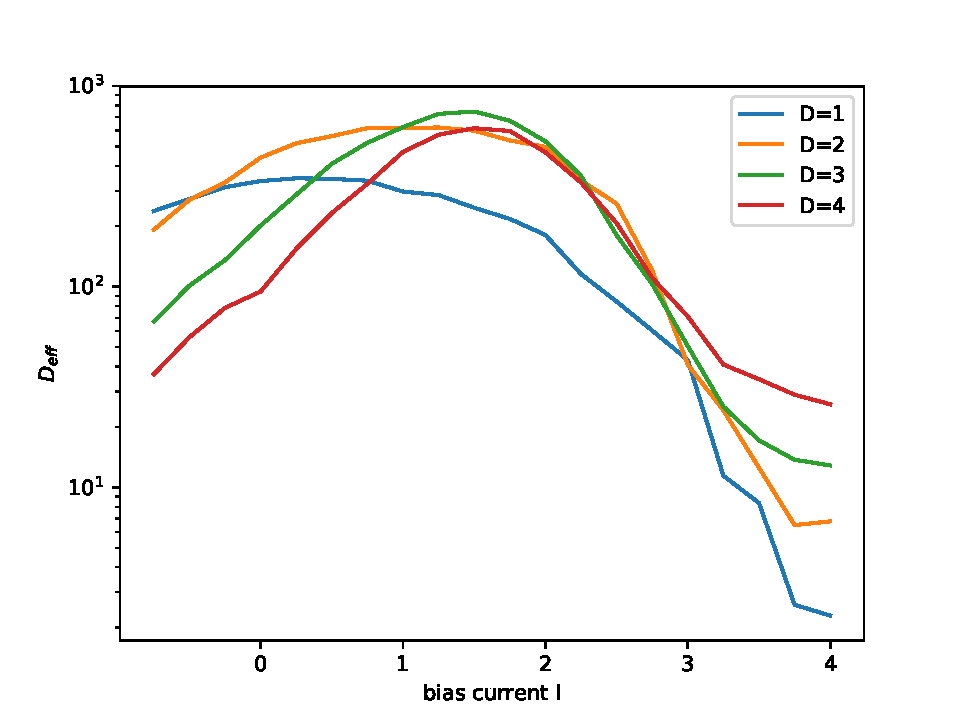
\includegraphics[scale=0.9]{dneur.pdf} 
	\caption{Diffusionskoeffizienten bei neuer Berechnung}
	\label{dn}
\end{figure} 
\begin{figure}[H]
	\centering
	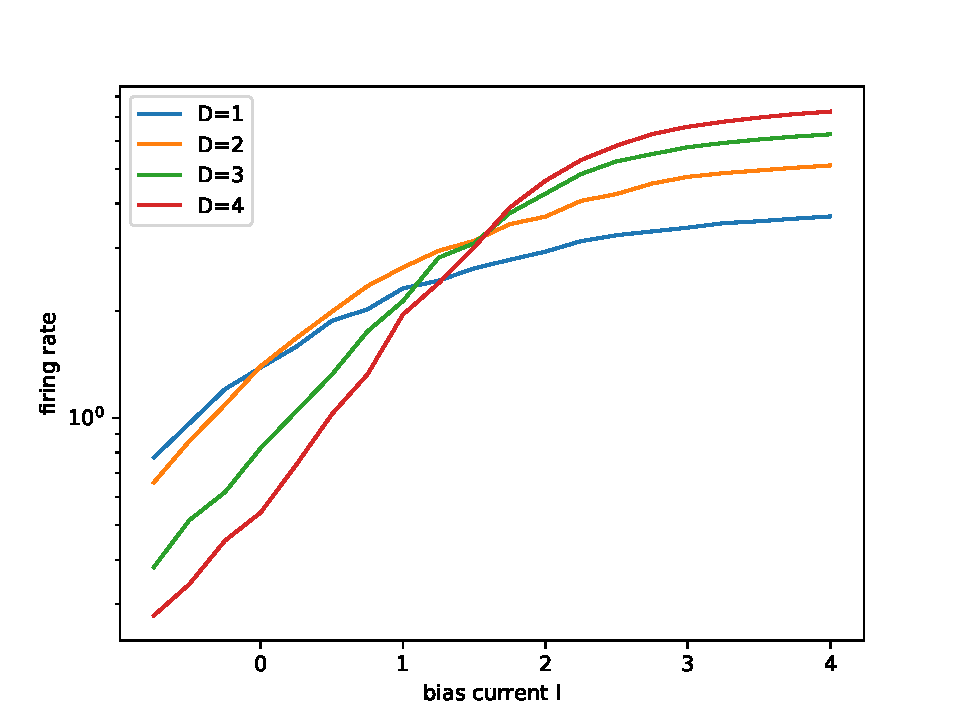
\includegraphics[scale=0.9]{gneur.pdf} 
	\caption{Feuerraten bei neuer Berechnung}
	\label{gn}
\end{figure} 
\begin{figure}[H]
	\centering
	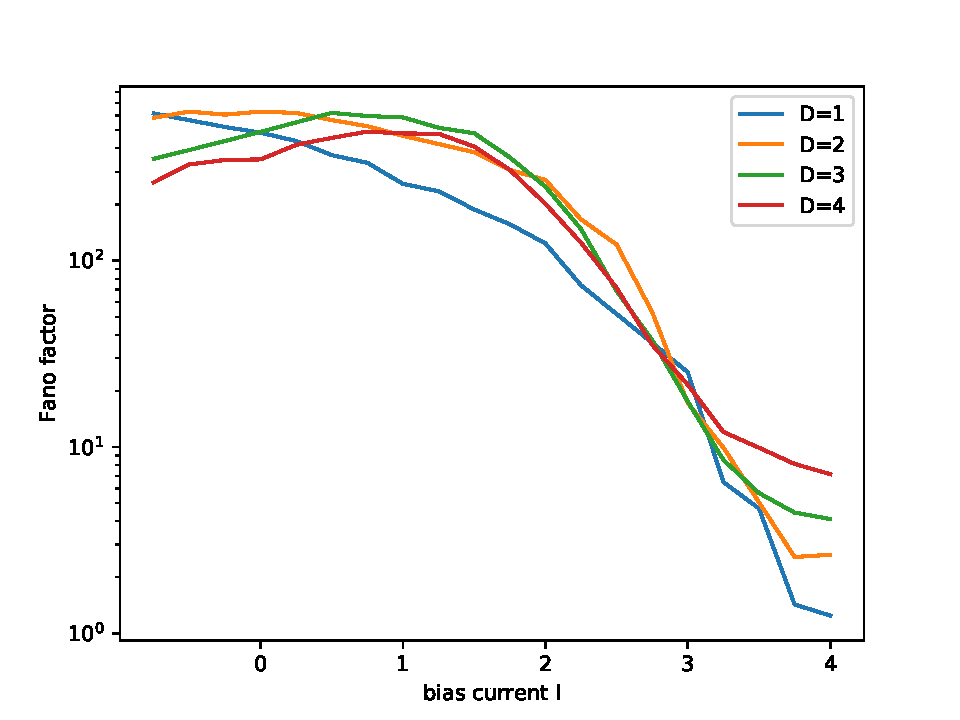
\includegraphics[scale=0.9]{fneur.pdf} 
	\caption{Fano-Faktoren bei neuer Berechnung}
	\label{fn}
\end{figure} 
Entgegen den ursprünglichen Beobachtungen zeigt die Geschwindigkeit das erwartete Verhalten, wie es die Phasendiagramme auch vermuten lassen. Offenbar hatten die ursprünglichen Simulationen noch nicht die notwendige Genauigkeit. Allerdings stehen noch einige Berechnungen für andere Werte von $D$ aus, die vielleicht das Bild noch verschieben könnten.\\
Überraschend fällt beim Betrachten von Diffusionskoeffizient und Fano-faktor auf, dass eine verringerte Rauschintensität nicht zu steigender Diffusion führt. \\
Weiteres Vorgehen: Erhöhung der Anzahl der Nervenzellen um eine Größenordnung (um damit hoffentlich eine akzeptable Genauigkeit zu erreichen) und Untersuchung von Rauschintensitäten $D<1$. Dabei auch Untersuchung auf Schnittstelle bei $I=3$. 
\section{mechanisches Modell}
Problem: es kann nicht die gewünschte Konvergenz erreicht werden. Wie im PRE wurde ein Zeitschritt von 0.01 gewählt.
%Hier sind drei Plots des gemittelten Diffusionskoeffizienten über Zeiten länger als $10^5$:
%\begin{figure}[H]
%\centering
%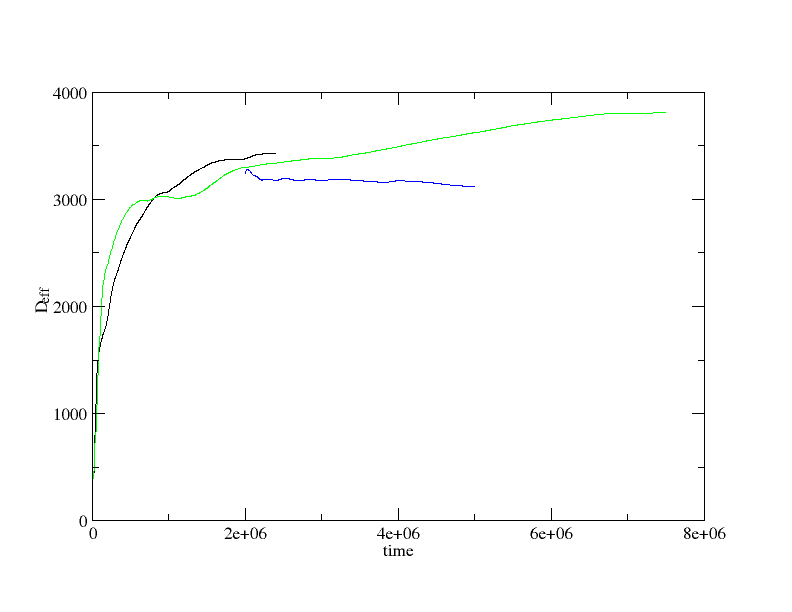
\includegraphics[scale=0.6]{mechcomp.png} 
%\caption{gemittelter Diffusionskoeffizient für verschiedene Laufzeiten; ab dem ersten Punkt des Plots wurde gemittelt; $kT=0.033$,$F=0.7$}
%\label{mc}
%\end{figure} 
%Der anhaltende Anstieg der beiden langen Graphen impliziert, dass zu früh mit dem Mitteln angefangen wurde. Obwohl der blaue Graph später gemittelt wurde, liegt er jedoch unter den beiden anderen Graphen. Die Rechnungen unterscheiden sich um m\\
Hier ist ein Vergleich von gemitteltem und tatsächlichem Diffusionskoeffizient

\begin{figure}[H]
	\centering
	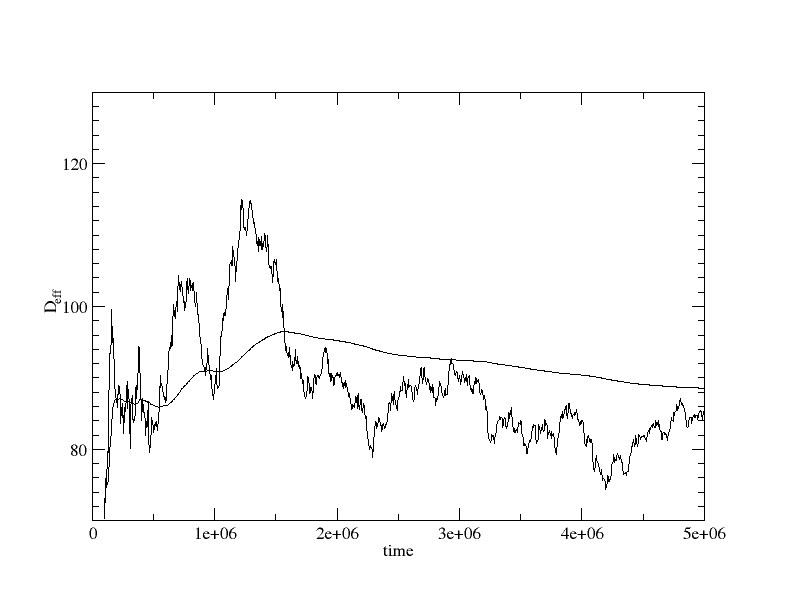
\includegraphics[scale=0.6]{deff94.png} 
	\caption{Vergleich gemittelter und tatsächlicher Diffusionskoeffizient; $kT=0.094$,$F=0.7$}
	\label{deff94}
\end{figure}
Auch nach $5\cdot10^6$ konvergiert der gemittelte Diffusionskoeffizient noch nicht.\\
Weiterhin habe ich hier zweimal die selbe Simulation laufen lassen, und kann keine komplett einheitlichen Ergebnisse erkennen:
\begin{figure}[H]
	\centering
	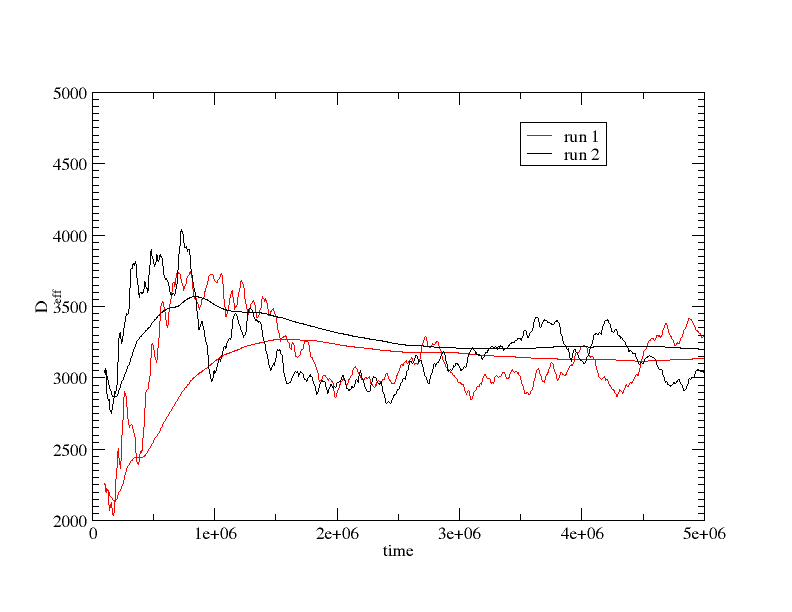
\includegraphics[scale=0.6]{deffcomp.png} 
	\caption{Vergleich gemittelter und tatsächlicher Diffusionskoeffizient für die selbe Rechnung; $kT=0.033$,$F=0.7$}
	\label{deffcomp}
\end{figure}
Auch nach 5 mal der im Paper angegebenen Laufzeit unterscheiden sich die beiden Kurven noch um wenige \%.\\

Lange Rede, kurzer Sinn, mit den angegebenen Konfigurationen lassen sich die Ergebnisse des Papers trotzdem relativ gut reproduzieren; die Rechnung für $kT=0.043$ wurde nur mit einer Zeit von $10^5$ durchgeführt; die Kurve für $kT=0.033$ wurde bereits mit $t_{max}=10^6$ ermittelt und die rechte Hälfte wird auch noch berechnet:
\begin{figure}[H]
	\centering
	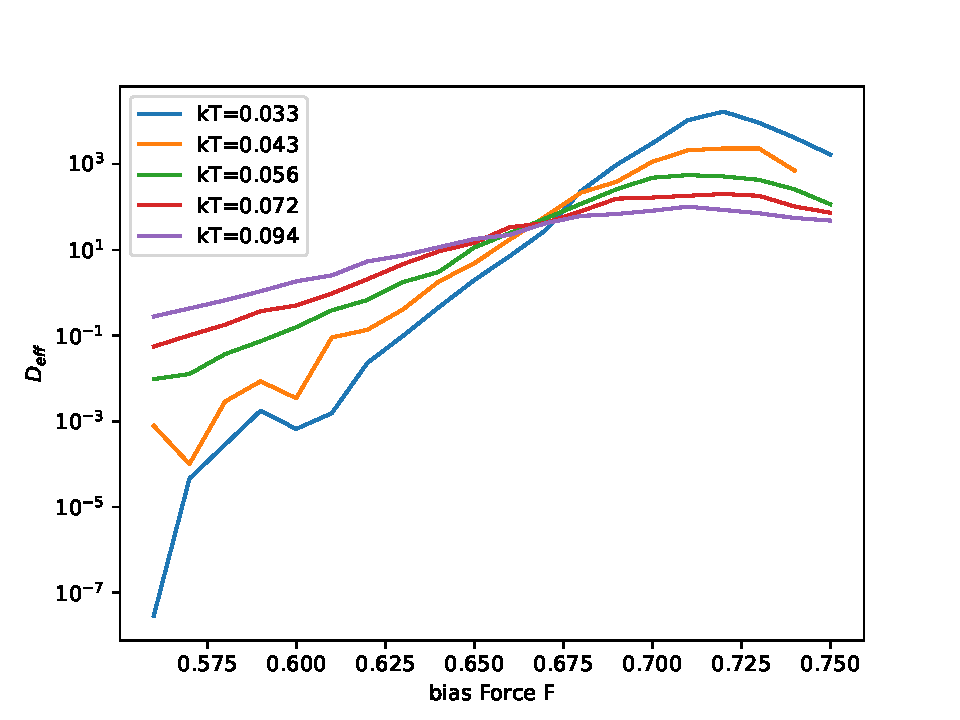
\includegraphics[scale=0.9]{mechdsh2.pdf} 
	\caption{Diffusionskoeffizienten für verschiedene Rauschintensitäten}
	\label{mdsh}
\end{figure}
\begin{figure}[H]
	\centering
	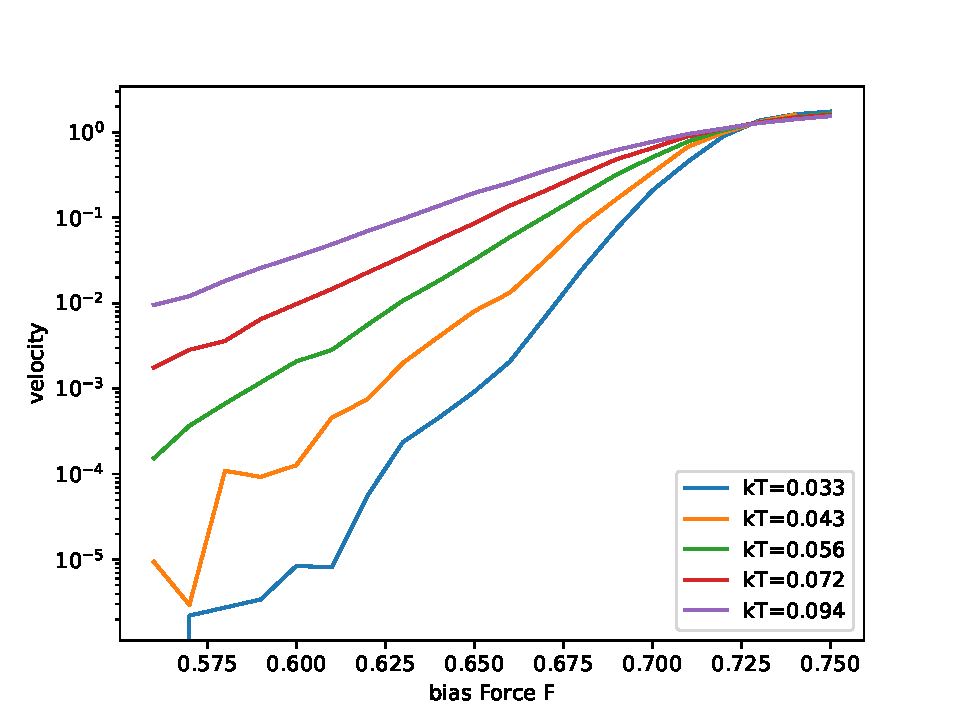
\includegraphics[scale=0.9]{mechgsh2.pdf} 
	\caption{mittlere Geschwindigkeiten für verschiedene Rauschintensitäten}
	\label{mgsh}
\end{figure}
\begin{figure}[H]
	\centering
	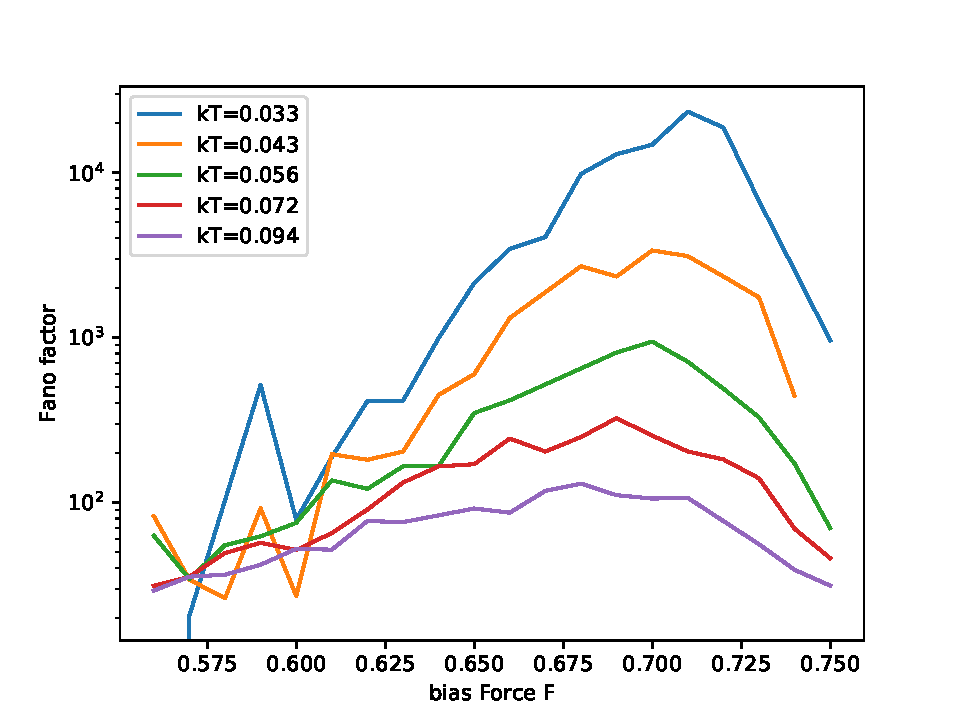
\includegraphics[scale=0.9]{mechfsh2.pdf} 
	\caption{Fano-Faktoren für verschiedene Rauschintensitäten}
	\label{mfsh}
\end{figure}
Weiteres Vorgehen: Fertigstellen der Rechnungen, evtl Überprüfen auf Schnittstellen, dann wird dieses Teilprojekt erstmal auf Eis gelegt.
\end{document}

